\documentclass[11pt]{article}
\usepackage[T1]{fontenc}
\usepackage{fontawesome}
\usepackage{lmodern}
\usepackage{parskip}
\usepackage[colorlinks=true,urlcolor=blue,linkcolor=black,citecolor=black]{hyperref}
\usepackage{graphicx}
\usepackage[utf8]{inputenc}
\usepackage[spanish]{babel}
\usepackage{fancyhdr}
\usepackage{csquotes}
\usepackage{lastpage}
\usepackage{array}
\usepackage[nottoc,numbib]{tocbibind}
\usepackage[activate={true,nocompatibility},final,tracking=true,kerning=true,spacing=true,factor=1100,stretch=10,shrink=10]{microtype}
\usepackage[hmargin=2cm,top=4cm,headheight=65pt,footskip=65pt]{geometry}


\graphicspath{{./pics/}}


\pagestyle{fancy}
\renewcommand{\headrulewidth}{0pt}
\fancyhead[CE,CO,LE,LO,RE,RO]{} %% clear out all headers
\fancyhead[C]{%
    \begin{tabular}{|m{4.5cm}|m{8.0cm}|m{4.5cm}|}
        \hline
        
\includegraphics[width=4.8cm]{logo2.png} &
        \centering
        \Large{Memoria del proyecto de evaluación extraordinaria} &
        \centering
        \normalsize{Página \thepage\ de \pageref{LastPage}}\tabularnewline
        \hline
    \end{tabular}%
    }
    \fancyfoot[CE,CO,LE,LO,RE,RO]{} %% clear out all footers
    %\fancyfoot[RE,LO]{}
    %\fancyfoot[LE,RO]{}
    \fancyfoot[C]{%
        \begin{tabular}{|m{7.5cm}|m{3.5cm}|m{6cm}|}
            \hline
            \normalsize{\textbf{Redactor:} Ángel García Menéndez}&
            \centering
            \normalsize{\textbf{Fecha:}\\15 de junio de 2020} &
            \normalsize{\textit{Software y Estándares para la Web}}\tabularnewline
            \hline
        \end{tabular}%
        }

        \title{Informe de la práctica}
        \author{Ángel García Menéndez}
        \date{15 de junio de 2020}

        \begin{document}

        \begin{titlepage}
            \centering
            
\includegraphics[width=0.25\textwidth]{logo}\par\vspace{1cm}
            {\scshape\LARGE Escuela de Ingeniería Informática de Oviedo\par}
            \vspace{1cm}
            {\scshape\Large Software y Estándares para la Web\par}
            \vspace{1.5cm}
            {\Huge\bfseries Memoria del proyecto de evaluación extraordinaria\par}
            \vspace{2cm}
            {\Large\itshape Ángel García Menéndez\par}
            {\Large\texttt{UO258654@uniovi.es}\par}
            \vfill

            % Bottom of the page
            {\large Curso 2019/2020\par}
        \end{titlepage}

        \tableofcontents
        \newpage
        \section{Introducctión}\label{intro}
        El presente trabajo tiene como objetivo servir como página web del IES Río Nora de la localidad asturiana de La Pola Siero.
        El sitio web cuenta con 4 páginas, siendo estas:
        \begin{itemize}
            \item El centro
            \item Los departamentos
            \item La biblioteca
            \item Actividades extraescolares
        \end{itemize}

        En todo momento se ha buscado primar la simplicidad y la claridad, ofreciendo un sitio sencillo y accesible, sin exceso de florituras, y con una estructura y diseños intuitivos.

        El proyecto se encuentra actualmente desplegado en la plataforma GitHub Pages a través del \href{https://flecktarn121.github.io/sew/extraordinary}{siguiente enlace}.

        \section{Consideraciones y modificaciones}
        El proyecto es en gran medida idéntico a la propuesta entregada en su momento, aunque determinados aspectos han podido variar, y determinadas acciones y decisiones requieren de ser expuestas y aclaradas.

        Por un lado, la API de GoogleMaps ha dado más problemas de los que debiera.
        Su comportamiento no es determinista, pues depende en gran medida de la localización del usuario.
        En principio funciona adecuadamente si se accede desde lugares situados en entornos urbanos, aunque esto no se puede asegurar.
        Uno de los usuarios con los que se realizaron las pruebas accedió desde su domicilio en \textit{La Felguera}, y no se le pudo procesar la ruta hasta el centro.
        Sin embargo, otro usuario desde \textit{Muros del Nalón} pudo hacer uso de esa funcionalidad sin ningún tipo de impedimento.

        Por otro lado, la implementación de los XML ha sido relativamente problemática.
        Al generarse el Schema se incluyeron una serie de directivas y espacios de nombres propios de Microsoft (se empleó Mono), y la validación del documento entraba en conflicto con la hoja de estilos XSLT.
        Básicamente, los espacios de nombres necesarios en la validación daban problemas a la hora de realizar la conversión a HTML.
        Finalmente se ha optado por ofrecer dos archivos XML, uno con la validación y otro con la conversión (ambos pueden accederse a través del sitio web, en el apartado \textit{Biblioteca}).

        Solo se ha recurrido a la etiqueta \texttt{div} en un caso, para la realización de la pequeña galería en el apartado \textit{Centro}.
        La razón de esto es que no se ha conseguido dar con una alternativa con más significado semántico para este caso concreto.
        Otra opción hubiese sido el empleo de imágenes sin más, saliendo pues perjudicada la usabilidad del sitio.
        Con esta salvedad, todo el sitio web hace uso del amplio abanico de etiquetas ofrecido por HTML5.

        \section{Estructura del proyecto}
        El proyecto se encuentra organizado en la siguiente jerarquía:

        \begin{itemize}
            \item \texttt{\faFolder{} img}: directorio de imágenes empleadas en el sitio web
            \item \texttt{\faFolder{} library}: directorio que alberga los XML relacionados con la biblioteca
                \begin{itemize}
                    \item \texttt{\faFileCodeO{} library-validated.xml}: archivo XML validado
                    \item \texttt{\faFileCodeO{} library.dtd}: archivo de validación mediante DTD
                    \item \texttt{\faFileCodeO{} library.xml}: archivo XML con hoja de estilos
                    \item \texttt{\faFileCodeO{} library.xsd}: archivo de validación mediante XML Schema
                    \item \texttt{\faFileCodeO{} library.xslt}: hoja de estilos XSLT
                \end{itemize}
            \item \texttt{\faFolder{} scripts}: directorio para los archivos ECMAScript del sitio web
                \begin{itemize}
                    \item \texttt{\faTerminal{} map.js}: script para la funcionalidad del mapa hacia el centro
                    \item \texttt{\faTerminal{} search.js} script que implementa la búsqueda de libros de la biblioteca
                    \item \texttt{\faTerminal{} weather.js} script que implementa la predicción meteorológica para el centro
                \end{itemize}
            \item \texttt{\faFolder{} vids}: directorio para los vídeos del sitio web
            \item \texttt{\faHtml5{} activities.html}: página de las actividades extraescolares
            \item \texttt{\faHtml5{} departments.html}: página de los departamentos del centro
            \item \texttt{\faHtml5{} index.html}: portada del sitio web, con la información del centro
            \item \texttt{\faHtml5{} library.html}: página sobre la biblioteca del centro
            \item \texttt{\faCss3{} style.css}: hoja de estilos del sitio web
        \end{itemize}

        \section{Pruebas}
        A continuación se exponen las diferentes pruebas con usurios realizadas.
        Se expondran los diferentes perfiles de las personas voluntarias, aunque sus datos personales se omitirán.

        \subsection{Primera tanda}
        Se procede a la recolección de opiniones sobre la estructura del sitio y presentación.

        \begin{itemize}
            \item \textbf{Nativo digital (no técnico)}: No tiene objeciones al respecto, aunque opina que la página tiene un estilo algo \textit{viejo} con respecto al aspecto que suelen ofrecer a día de hoy.
            \item \textbf{Nativo digital (técnico)}: Bastante contento con lo ofrecido, especialmente con la combinación de colores.
            \item \textbf{Adulto no nativo digital}: Cree que el SVG necesitaría presentarse de otra forma, sobretodo la colocación de los nombres y los números.
            \item \textbf{Adulto de poca destreza digital}: No encuentra especial problemática. Necesita recolocar la pantalla para leer.
        \end{itemize}

        \subsubsection{Soluciones planteadas}
        Se pasa a cambiar la colocación del SVG de vertical a horizontal, invirtiendo asimismo la posición del texto con los números.

        Se aumenta ligeramente el tamaño de letra.

        \subsection{Segunda tanda}
        Se procede a comprobar si la funcionalidad del mapa tiene el comportamiento esperado.

        \begin{itemize}
            \item \textbf{Nativo digital (no técnico)}: Le aparece el mapa y se le muestra la ruta con normalidad.
            \item \textbf{Nativo digital (técnico)}: No aparece el mapa.
                Al pulsar el botón de \textit{Generar ruta} surge un error de localización, mostrándose finalmente el mapa, pero sin la ruta al centro.
            \item \textbf{Adulto no nativo digital}: Problema similar al anterior sujeto.
            \item \textbf{Adulto de poca destreza digital}: El comportamiento de la funcionalidad es completamente normal.
        \end{itemize}

        \subsubsection{Soluciones planteadas}
        Este parece ser un problema propio de los servicios de Google, parece ser que depende en gran medida de la localización geográfica del usuario en el momento de hacer uso del servicio.
        No se encuentra ninguna solución plausible.

        \subsection{Tercera tanda}
        Se le enumera a los usuarios los contenidos de la biblioteca y se les pide que comprueben si está disponible uno de los ejemplares.

        \begin{itemize}
            \item \textbf{Nativo digital (no técnico)}: Necesita de un par de lecturas de la página correspondiente hasta que encuentra el buscador.
                Realiza la búsqueda con éxito.
            \item \textbf{Nativo digital (técnico)}: Encuentra a la primera el buscador y hace uso del mismo para obtener la información.
            \item \textbf{Adulto no nativo digital}: Hace uso del buscador, aunque tarda dos intentos en hacerlo de forma exitosa.
            \item \textbf{Adulto de poca destreza digital}: Lee con detenimiento la página y accede al catálogo completo de la biblioteca (el XML con la transformación en HTML) por el enlace que se le ofrece justo antes del buscador.
        \end{itemize}

        \subsubsection{Soluciones planteadas}
        Se trata de una de las funcionalidades más complejas, y para obtener un comportamiento 100\% satisfactorio sería necesario crear un motor de búsqueda que escapa al alcance de lo que se plantea en el presente proyecto.

        \section{Resultados de los validadores}
        A continuación se exponen los resultados de los validadores y las soluciones a los problemas encontrados.
        Las capturas de pantalla se encuentran en los anexos respectivos al final del documento.

        \subsection{Validadores del W3C}
        Se somete a los validdores del World Wide Web Consortium tanto a los 4 documentos HTML como a la hoja de estilos.
        En todos los casos los resultados son satisfactorios, no generándose ningún tipo de error o advertencia.

        Se pueden comprobar los resultados haciendo uso de los botones en el pié de las páginas.

        \subsection{Validadores de accesibilidad}

        El validador \textbf{Wave} ofrece resultados normales, a excepción de dos problemas.
        El primero es una ligera advertencia por la lentitud al cargar el vídeo en el apartado de los departamentos, y el otro es un error en toda regla por la ausencia de una \textit{label} en el campo de texto del buscador.

        \textbf{AChecker} también presenta la problemática del campo de texto del buscador.

        Misma situación en \textbf{TAW}, amén de advertencias generadas por el carácter automático de la herramienta.

        Se añade la \textit{label} necesaria en el buscador de la biblioteca.

        \subsection{Validadores de adaptabilidad}
        Se prueban diferentes convinaciones de pantallas en \textbf{Screenfly} y \textbf{Responsive Design Checker}.
        En ambos casos la página se adapta correctamente, aunque las resoluciones más pequeñas sí que tienen un impacto apreciable.

        \textbf{Google Mobile Friendly} da el visto bueno a todos los documentos, ofreciendo algunas advertencias por la carga de determinados contenidos (como el mapa de la portada o la previsión meteorológica).

        \clearpage{}

        \section{Anexos}
        \subsection{Validadores de accesibilidad}

\begin{figure}[h]
    \centering
    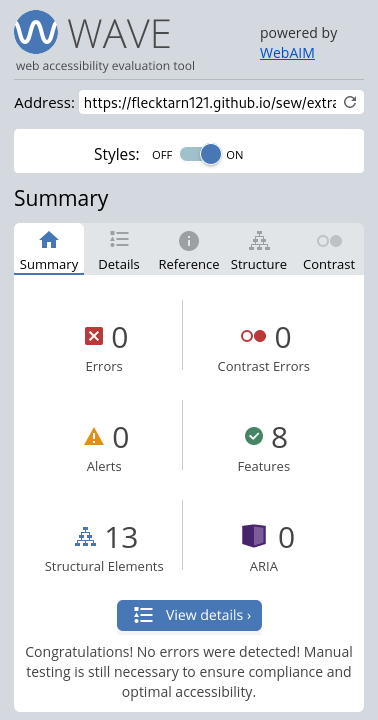
\includegraphics[width=0.4\textwidth]{wave1.png}
    \caption{Resultados de Wave para la portada}
\end{figure}

\begin{figure}[h]
    \centering
    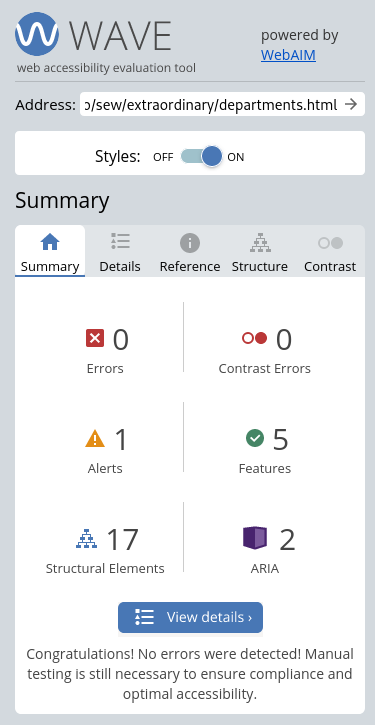
\includegraphics[width=0.4\textwidth]{wave2.png}
    \caption{Resultados de Wave para los departamentos}
\end{figure}

\begin{figure}[h]
    \centering
    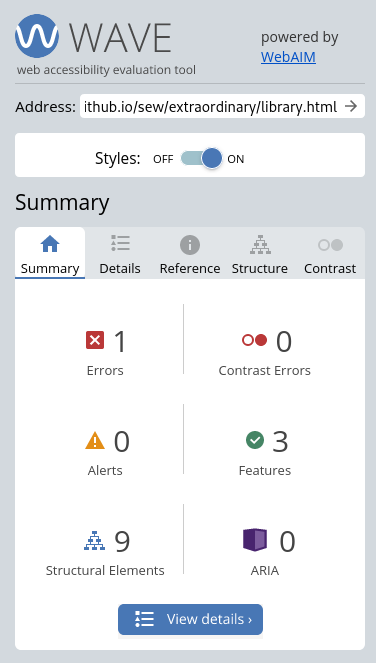
\includegraphics[width=0.4\textwidth]{wave3.png}
    \caption{Resultados de Wave para la biblioteca}
\end{figure}

\begin{figure}[h]
    \centering
    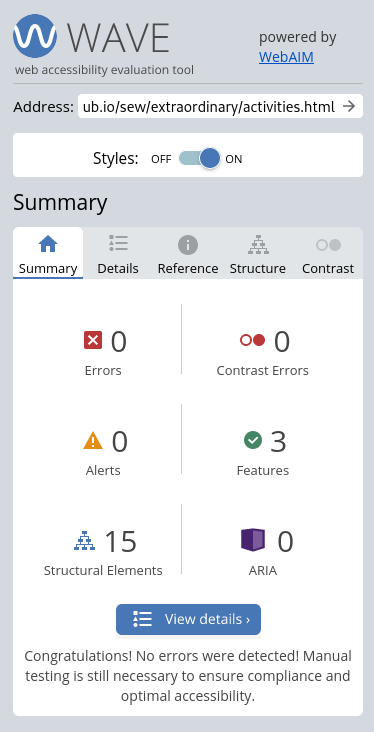
\includegraphics[width=0.4\textwidth]{wave4.png}
    \caption{Resultados de Wave para las actividades}
\end{figure}

\begin{figure}[h]
    \centering
    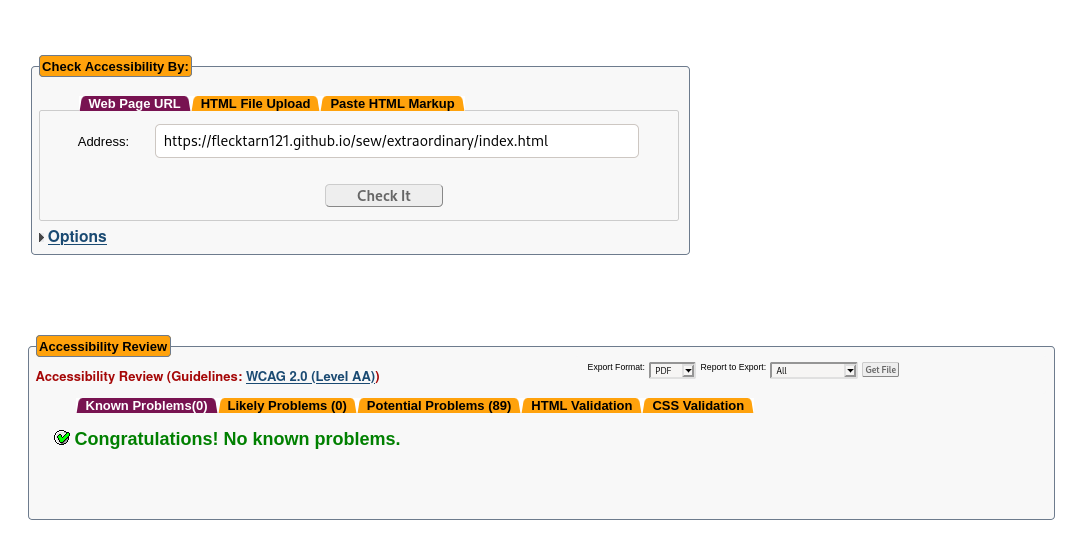
\includegraphics[width=0.85\textwidth]{achecker1.png}
    \caption{Resultados de aChecker para la portada}
\end{figure}

\begin{figure}[h]
    \centering
    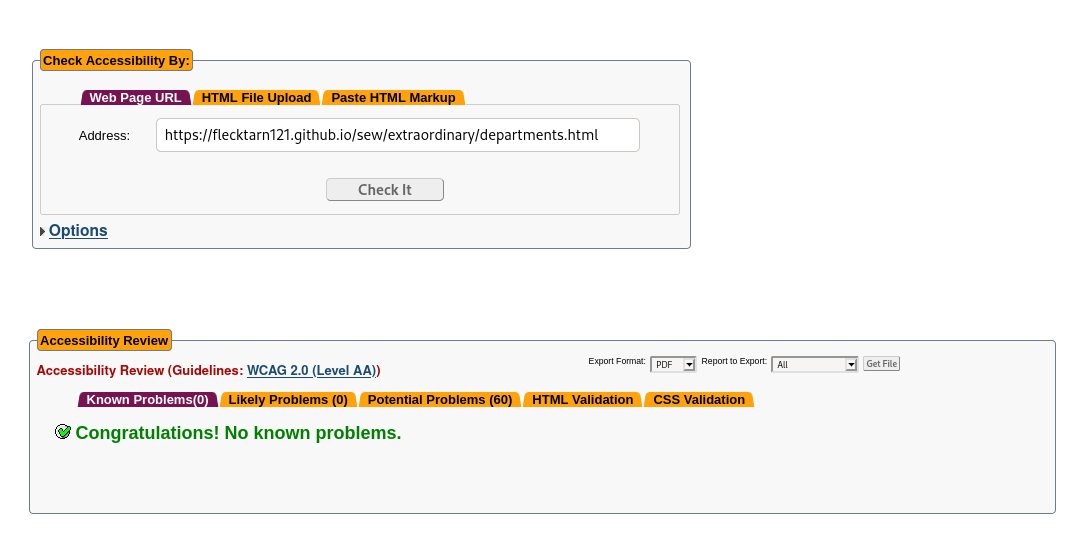
\includegraphics[width=0.85\textwidth]{achecker2.png}
    \caption{Resultados de aChecker para los departamentos}
\end{figure}

\begin{figure}[h]
    \centering
    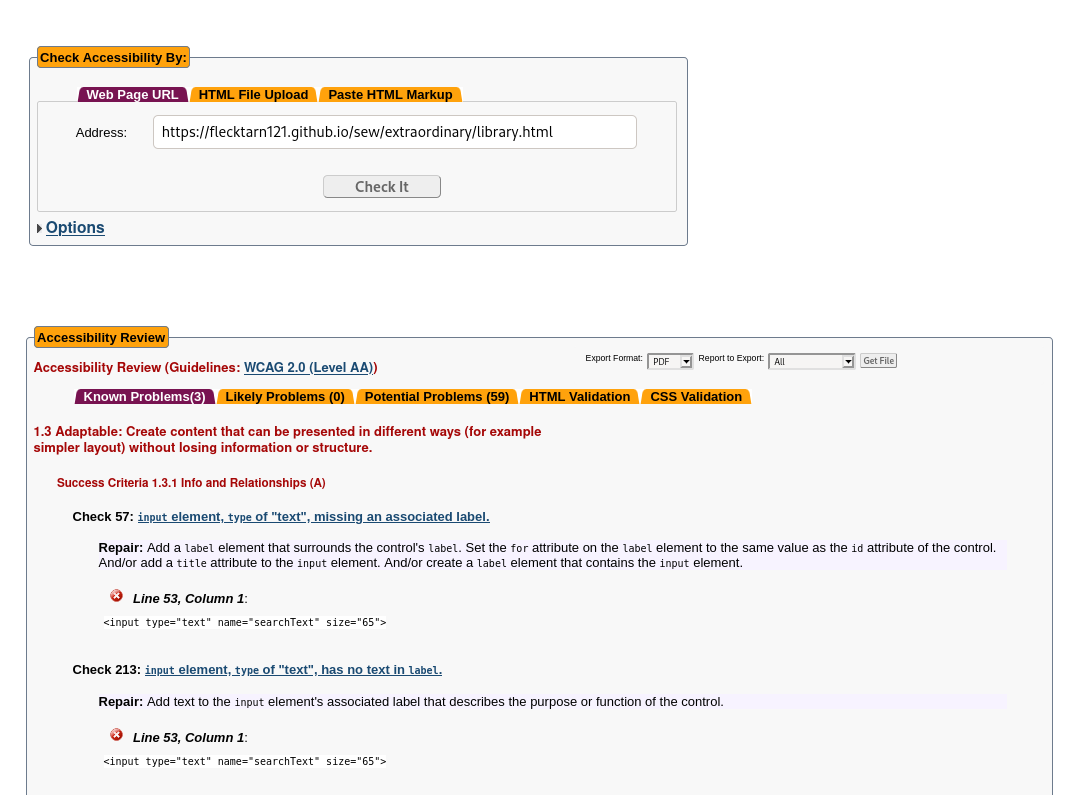
\includegraphics[width=0.85\textwidth]{achecker3.png}
    \caption{Resultados de aChecker para la biblioteca}
\end{figure}

\begin{figure}[h]
    \centering
    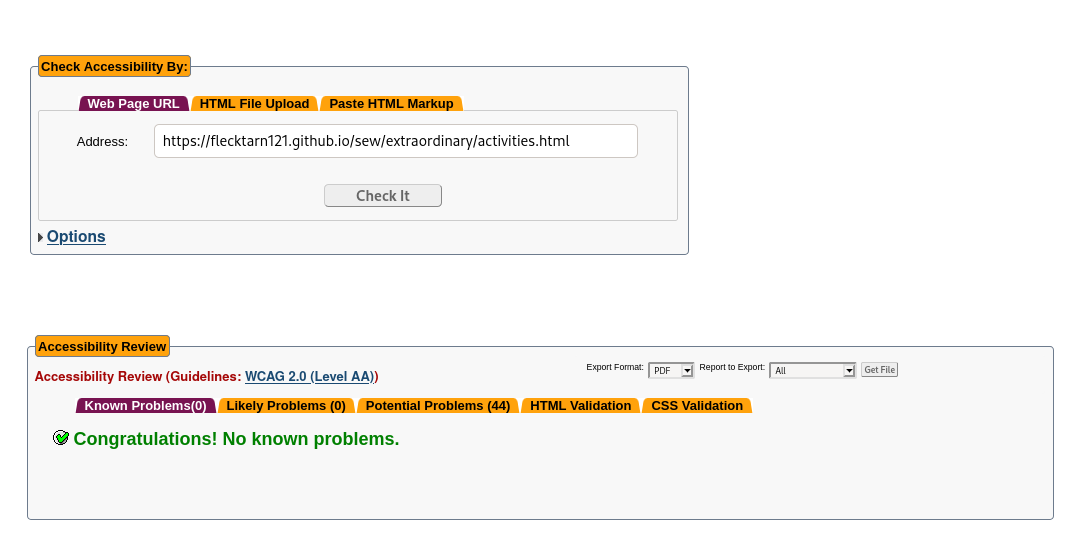
\includegraphics[width=0.85\textwidth]{achecker4.png}
    \caption{Resultados de aChecker para las actividades}
\end{figure}


\begin{figure}[h]
    \centering
    
\includegraphics[width=\textwidth]{taw1.png}
    \caption{Resultados de TAW para la portada}
\end{figure}

\begin{figure}[h]
    \centering
    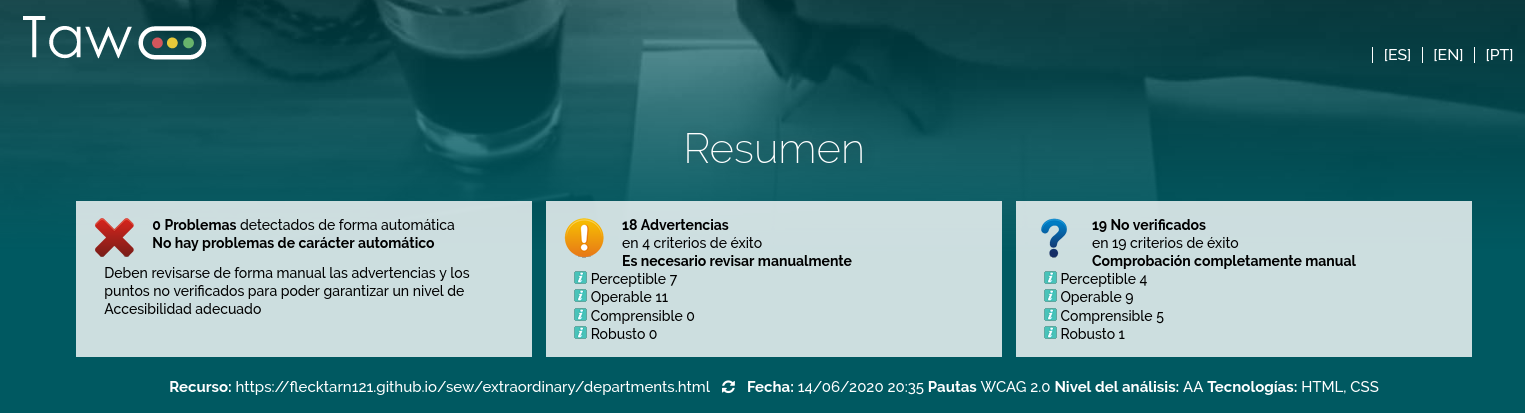
\includegraphics[width=\textwidth]{taw2.png}
    \caption{Resultados de TAW para los departamentos}
\end{figure}

\begin{figure}[h]
    \centering
    
\includegraphics[width=\textwidth]{taw3.png}
    \caption{Resultados de TAW para la biblioteca}
\end{figure}

\begin{figure}[h]
    \centering
    
\includegraphics[width=\textwidth]{taw4.png}
    \caption{Resultados de TAW para las actividades}
\end{figure}

\clearpage{}

\subsection{Validadores de adaptabilidad}

\begin{figure}[h]
    \centering
    
\includegraphics[width=0.45\textwidth]{screenfly.png}
    \caption{Simulación en Screenfly de la página en móviles}
\end{figure}

\begin{figure}[h]
    \centering
    
\includegraphics[width=0.75\textwidth]{responsive-design-checker.png}
    \caption{Simulación en Responsive Design Checker de la página en móviles}
\end{figure}

\begin{figure}[h]
    \centering
    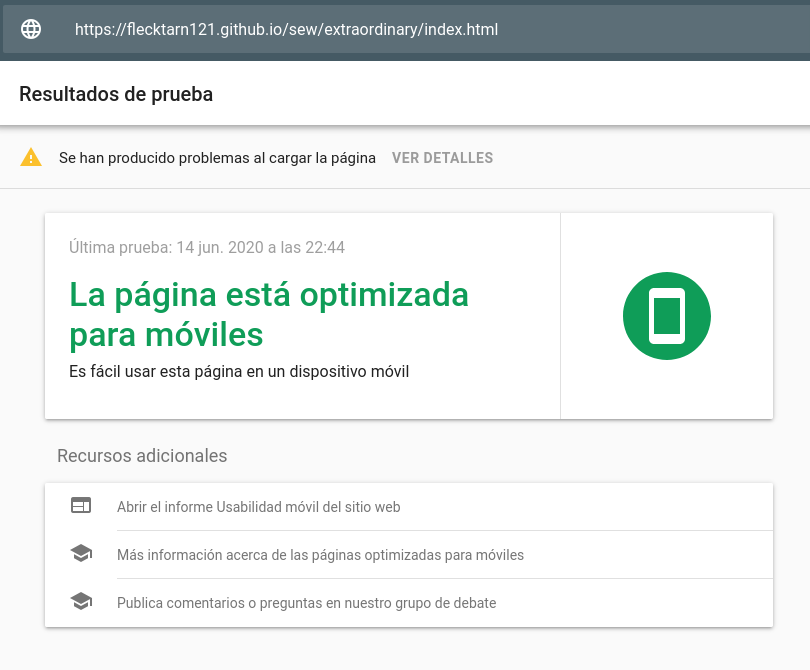
\includegraphics[width=0.75\textwidth]{google1.png}
    \caption{Resultados de adaptabilidad de Google para la portada}
\end{figure}

\begin{figure}[h]
    \centering
    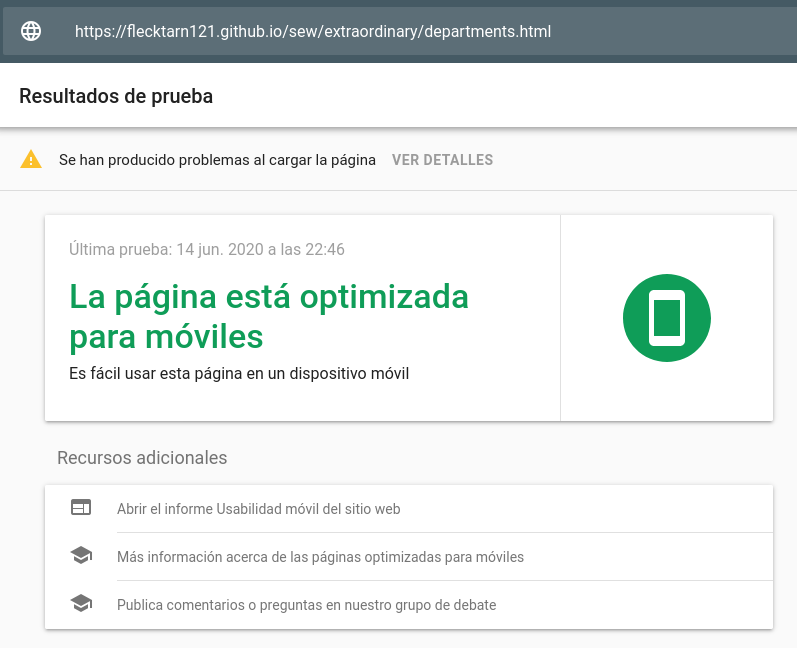
\includegraphics[width=0.75\textwidth]{google2.png}
    \caption{Resultados de adaptabilidad de Google para los departamentos}
\end{figure}

\begin{figure}[h]
    \centering
    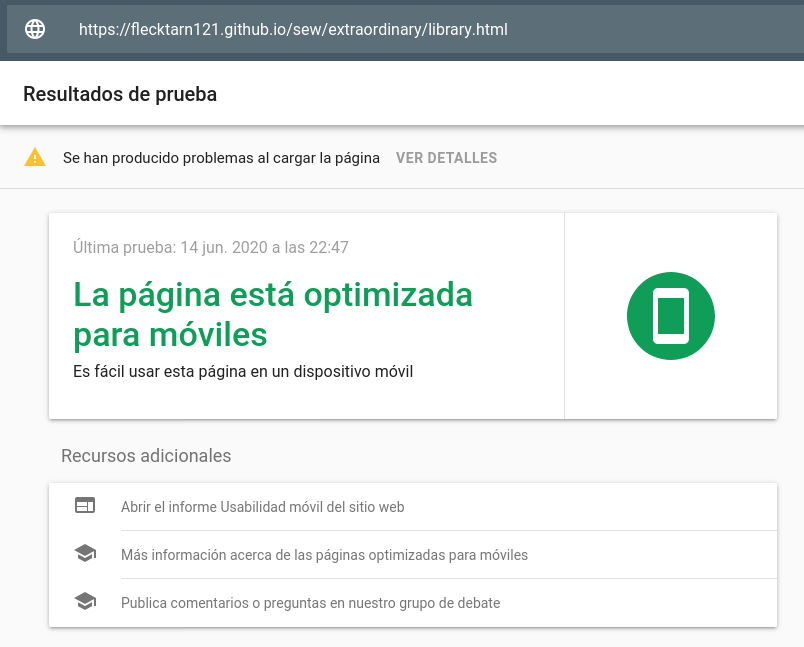
\includegraphics[width=0.75\textwidth]{google3.png}
    \caption{Resultados de adaptabilidad de Google para la biblioteca}
\end{figure}

\begin{figure}[h]
    \centering
    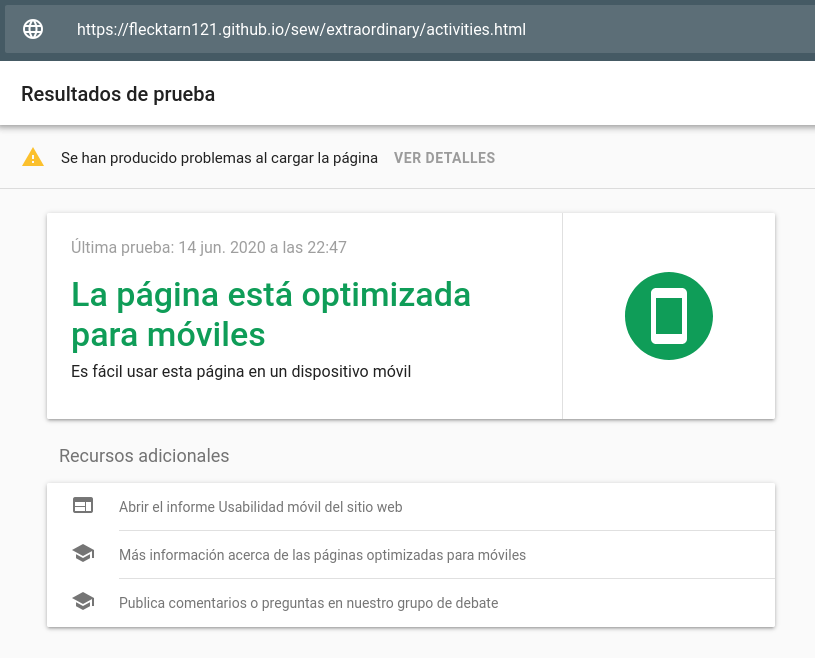
\includegraphics[width=0.75\textwidth]{google4.png}
    \caption{Resultados de adaptabilidad de Google para las actividades}
\end{figure}

        \end{document}
